\documentclass{article}
\usepackage[utf8]{inputenc}

\author{Accordi Gianmarco}
\title{Reverse Engineering}

\usepackage{natbib}
\usepackage{graphicx}
\usepackage{minted}
\usepackage{tabularx}
\usepackage{tikz}
\usepackage{pgfplots}
\usepackage{hyperref}

\usemintedstyle{fruity}
\date{}

\begin{document}

\maketitle

\section{Introduction}

\textbf{Reverse Engineering} is the process of understanding how system made by man is working, by looking at it an trying to reverse the operations it does in order to understand its behavior.
Its like a scientific research but in this case we are not interested in natural phenomenon.
This kind of process has been applied to a lot of different fields, from mechanical engineering to chemical engineering, so as the name suggested it is applied to all field of engineering: these are the fields in which we can take apart the work done by other human being and trying to understand how they have build such a system.
The necessity of this such an analysis of a system is usually required because creator of a system tends to disclose how they've built it, this mean that they obscure their work in order to protect their creators rights.
The purpose of this document is to give an introduction on \textbf{Reverse Engineering} specifically in the field of Software Engineering.
The process of Reverse Engineering applied to Software products can be done at any level of the production, but it usually involves two stages:
\begin{itemize}
    \item \textbf{Redocumentation}: since usually the given software product that we want to analyze is already compiled we want to be able to reach an higher level of abstraction to better understand the code;
    \item \textbf{Design Understanding}: once that we have been able to get an higher abstraction of our code we can use our capacity and knowledge in order to understand what the program does and how it does it, so we want to follow the development process of the creators of such code.
\end{itemize}
Disclose the design features can be conducted with two approaches:
\begin{itemize}
    \item \textbf{Dynamic Analysis}: this is an on the field approach, in which you launch the program and you register what the program is doing, and by analyzing the impact it has on the environment(print,systemcalls,...) you try to figure out what it does;
    \item \textbf{Static Analysis}: analyze the code without launch it, you analyze only the output you've obtained from the \underline{Redocumentation} part.
\end{itemize} 
In next sections we will analyze this approaches along with the stage involved in doing them.
Then we proceed in order to define which is the best strategy based on what we have seen. Finally an example is provided taken from a CTF. 

\subparagraph{Reverse Engineering in Software Engineering}
As previously stated this document focus its attention on Reverse Engineering applied to software. When a new software is released it is usually provided already compiled to the specific architecture, so you get the binary of this code.
The binary, as the name suggests, contains binary instructions that are targeted to be understood by a specific machine with a specific architecture, this means that it cannot be understand easily from a human being.
For the developers this is usually a wanted feature, since this make the reverse engineering process more difficult for other companies that wants to disclose their design features.
To be even more secure companies also rely on the usage of some \underline{Obfuscation Technique} that makes the reverse engineering process even harder. This leads to the development of new research fields focused on trying to remove obfuscation, also in an automate way \citep{1566145}.
Some techniques used for obfuscate binaries are Packing( in which the source code pack and unpack the .text section as long as it execute)\citep{SlidePackers}, Dynamic Code Mutation( in which the code mutate during execution), Code Generation( the program generates code during program execution) or by Binary Instumentation \cite{paperInstrumentation}.
So in the end software is usually not fully disclose for two main reasons: protection of intellectual property and malware. In next sections we will see different techniques that can be used in order to defeat make the process of reverse engineering more easy.
As a small note the fact that usually companies tends not to disclose their code leads to problem in computer security, since it cannot be reviewed from external person in order to find security problems. Such way of thinking is changing in recent days \citep{articleOpensource}.

\section{Stages}

\subsection{Redocumentation}
The program we get is usually a binary file so the first steps in order to get an higher level representation of it is to disassemble it 
\begin{figure}[tbh]
    \centering
    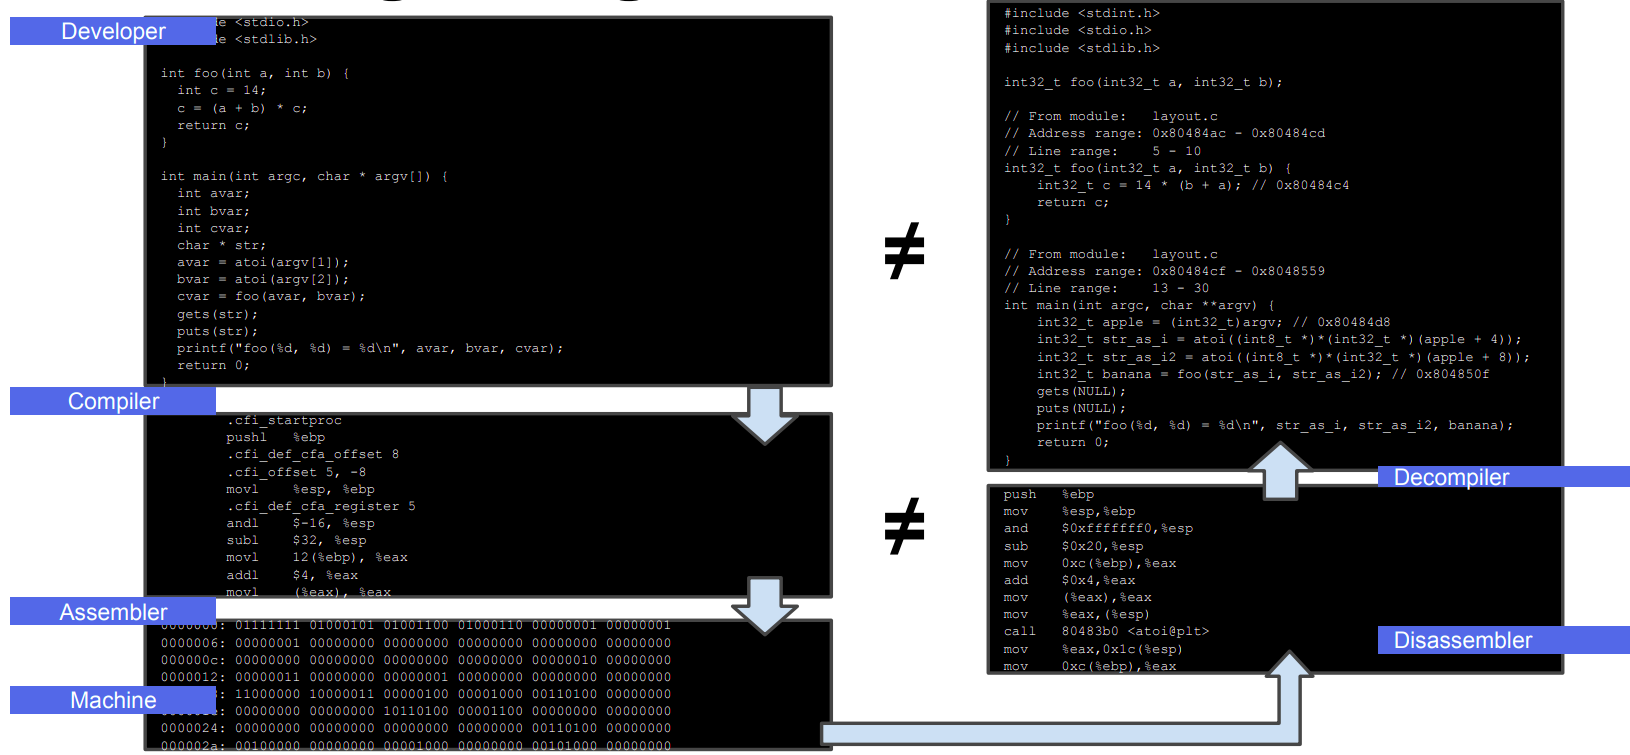
\includegraphics[width=1\textwidth]{images/disassembe.png}
    \caption{Compilation and Decompilation steps\citep{SlideReverse}}
    \label{fig:universe}
\end{figure}



If you need a reference to a link please use footnotes\footnote{\url{https://jinblack.it}}. If you are referencing to a paper or book you the bibliografy.
Use texttt when refering to register name or code in general like \texttt{EIP} or \texttt{call}

You can start from this example to build your report. Include in your final submission all the source code needed to perform any edit in the future including images source as well.

\begin{figure}[tbh]
\centering
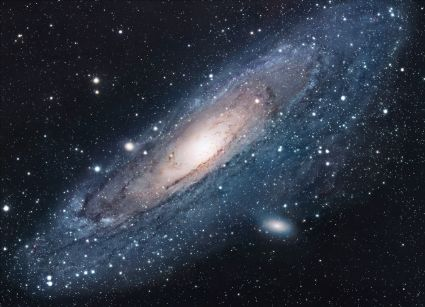
\includegraphics[width=0.7\textwidth]{images/universe.jpg}
\caption{Img example}
\label{fig:universe}
\end{figure}

\begin{figure}[tbh]
\centering
\usetikzlibrary{shapes.multipart,calc, positioning,patterns,backgrounds}
\makeatletter
\newcommand{\gettikzxy}[3]{%
  \tikz@scan@one@point\pgfutil@firstofone#1\relax
  \edef#2{\the\pgf@x}%
  \edef#3{\the\pgf@y}%
}
\makeatother

\begin{tikzpicture}[stack/.style={rectangle split, rectangle split parts=#1,draw, anchor=center},scale=0.65, transform shape]
\node(s)[stack=14]  {
\nodepart{one}   \vdots    % text
\nodepart{two}   \ttfamily sub ecx, 1     % text
\nodepart{three}   \ttfamily jmp 0x75000014     % two
\nodepart{four} \vdots     % three
\nodepart{five}  \ttfamily 0x04000012 % four
\nodepart{six} \vdots
\nodepart{seven} \ttfamily add eax, 4
\nodepart{eight} \ttfamily mov ebx, [esp]
\nodepart{nine} \ttfamily jmp 0x04001000
\nodepart{ten} \vdots
\nodepart{eleven} \ttfamily pop ebp
\nodepart{twelve} \ttfamily push eax
\nodepart{thirteen} \ttfamily jmp 0x03a4a5a6
\nodepart{fourteen} \vdots
};

\node(q)[stack=9, right=2cm of s]  {
\nodepart{one}   \vdots    % text
\nodepart{two}   \ttfamily add eax,4     % two
\nodepart{three}  \ttfamily mov ebx, [esp]     % three
\nodepart{four}  \ttfamily pop ebp % four
\nodepart{five}  \ttfamily push eax
\nodepart{six} \ttfamily sub ecx,1
\nodepart{seven} \ttfamily MessageBox() + 0x14
\nodepart{eight} \ttfamily MessageBox() + 0x18
\nodepart{nine} \vdots
};

% Adding comments and pointers
\draw[<-,>=stealth](s.two west)--+(-20pt,0pt) node[anchor=east, align=left]{\footnotesize \ttfamily 0x03a4a5a6};
\draw[<-,>=stealth](s.five west)--+(-20pt,0pt) node[anchor=east,text width=1.8cm,align=left]{\footnotesize {\ttfamily 0x04000000} \newline IAT entry};
\draw[<-,>=stealth](s.seven west)--+(-20pt,0pt) node[anchor=east, align=left]{\footnotesize \ttfamily 0x04000012};
\draw[<-,>=stealth](s.eleven west)--+(-20pt,0pt) node[anchor=east, align=left]{\footnotesize \ttfamily 0x04010000};
\draw[->,>=stealth, dashed](s.five east) --+(10pt, 0)  --  node[anchor=west] {1} ([shift=({10pt,0})]s.seven east) -- (s.seven east);
\draw[->,>=stealth, dashed](s.eight east) --+(10pt, 0)  --  node[anchor=west] {2} ([shift=({10pt,0})]s.eleven east) -- (s.eleven east);
\draw[->,>=stealth, dashed](s.thirteen east) --+(25pt, 0)  --  node[anchor=west] {3} ([shift=({25pt,0})]s.two east) -- (s.two east);

%Get x and y coordinates of point A
\gettikzxy{(s.three east)}{\ax
}{\ay}
\gettikzxy{(q.seven west)}{\bx}{\by}

\draw[->,>=stealth, dashed](s.three east) -- (\ax+40pt, \ay)  --  node[anchor=west] {4} (\ax+40pt, \by) -- (q.seven west);

\draw[<-,>=stealth](q.two east)--+(+20pt,0pt) node[anchor=west,text width=2cm,align=left]{\footnotesize {\ttfamily 0x75000000} \newline Entry point MessageBox API};


   \begin{pgfonlayer}{background}
       \draw[pattern=vertical lines, pattern color=red!50] (s.two split east) rectangle (s.one split west);
       \draw[pattern=vertical lines, pattern color=red!50] (q.six split east) rectangle (q.five split west);

       \draw[pattern=north west lines, pattern color=yellow!60] (s.eight split east) rectangle (s.six split west);
       \draw[pattern=north west lines, pattern color=yellow!60] (q.text split east) rectangle (q.three split west);


       \draw[pattern=horizontal lines, pattern color=green!60] (s.ten split east) rectangle (s.twelve split west);
       \draw[pattern=horizontal lines, pattern color=green!60] (q.three split east) rectangle (q.five split west);


%       \draw[pattern=dots, pattern color=blue!60] (e.text split west) rectangle (e.two split east);
 %      \draw[pattern=horizontal lines, pattern color=olive!60] (e.two split west) rectangle (e.three split east);
  %     \draw[pattern=vertical lines, pattern color=magenta!60] (e.three split west) rectangle (e.south east);
    \end{pgfonlayer}


\end{tikzpicture}
 \caption{You can use tikz to draw nice memory drawing (example in file \texttt{stack\_representation\_example.pgf}.). Or google draw.  If you use other tools, make sure to have all figure as \texttt{pdf}. Moreover, if you use an external tool, make sure to provide a way to modify the produced images. A link to google draw with correct permission is good enough.}
\label{general-stolen-api}
\end{figure} 


\subsection{Example of code}
Here you can fine an example of how to add some code. It is using the package minted with basic option enabled.
You can write code in place:
\begin{minted}[linenos, bgcolor=black, escapeinside=!!]{python}
import numpy as np
    
def incmatrix(genl1,genl2):
    m = len(genl1)
    n = len(genl2) !\label{myline}!
    M = None #to become the incidence matrix
    VT = np.zeros((n*m,1), int)  #dummy variable
    
    #compute the bitwise xor matrix
    M1 = bitxormatrix(genl1)
    M2 = np.triu(bitxormatrix(genl2),1) 
...
\end{minted}
You can reference to a line
The important line is line \ref{myline}.

You can use an external file and ave the code as listing.
\begin{listing}[ht]
\inputminted[linenos, bgcolor=black, escapeinside=!!]{python}{x.py}
\caption{Example from external file}
\label{listing:3}
\end{listing}
 
The important line is line \ref{anotherline} of Listing~\ref{listing:3}.

\section{Conclusion}


\bibliographystyle{plain}
\bibliography{references}
\end{document}
